% Chapter 4
\chapter{Transmission Expansion Planning by Quantum Annealing} % Main chapter title
\label{Chapter4} % For referencing the chapter elsewhere, use \ref{Chapter1} 
\section{Statement of the Problem}
The \textit{Transmission expansion planning} (TEP)\,\cite{Neumann2020TransmissionFlows} problem determines the number of new lines to be installed in order to achieve a specific goal, optimizing the performance of an energy system subject to the assumptions of a future scenario. It is classically formulated as a \textit{mixed integer linear programming} (MILP) problem that aims at finding the optimal way to expand the capacity of an energy system by minimizing the cost function, which is the sum of the investment cost of transmission lines and the operational cost of generators. It decides how many transmission lines to build and where to connect them in order to satisfy the energy demand on a distributed energy system with a high share of renewable energy sources. There are other components to build apart from transmission lines such as generators or storages, but considering them implies not only an increment in the number of variables of the problem but also an increment in its complexity. For this reason, the problem we are solving is not completely realistic but it encapsulates the most important features of it. We should consider it just as a starting point to get insight about the problem formulation and challenges.\\\\
We can control the number of variables of the problem according to
\begin{itemize}
    \item \textbf{Number of nodes:} clustering techniques allow us to fix the number of nodes of the problem so that some loads of a given network are grouped acting as a single big load.
    \item \textbf{Snapshots of time}: in expansion problems it is common to consider hourly snapshots of time of one year, i.e., a total of 8760 snapshots. However, we can restrict the problem to a subset of snapshots without loss of generality.
    \item \textbf{Connectivity of transmission lines}: we can control the connectivity between nodes so that we do not allow a node the possibility of being fully connected with the rest of nodes. Furthermore, because of legal procedures to build new lines in areas where there are no transmission lines, TEP focuses on building lines in existing connections without changing the topology of the network.
    \item \textbf{Adding targets}: in this chapter we minimize the cost function as function of the investment cost of transmission lines, operational cost of generators and the load shedding cost, which is going to be explained later. But, there are other targets such as the increment of renewable energy sources in a given region or the reduction of the carbon footprint that we are not taking into account.
\end{itemize}
The resolution of MILP associated to TEP scales badly using classical algorithms\,\cite{Oertel2014ComplexityEvaluation} and, at the same time, energy system models are getting larger and more complex due to the integration of decentralized weather-dependent renewable energy sources, intermittent loads, sector coupling and the increase of storage components. Currently, the problem is often linearized or the scope and granularity of the model are reduced using clustering algorithms. For this reason, any computational time reduction will have substantial implications in closing the granularity gap between what the current models can solve and the desired resolution needed by energy system operators. However,  since quantum computers are still not sufficiently mature, large TEP problems cannot be solved fully by a quantum annealer. For this reason, we require hybrid methods\,\cite{Dilwali2016,Binato2001,Huang2019,MacRae2016,Zhao2021HybridProgrammingb} to decompose large problems into a master problem, which can be solved by a quantum annealer, and a sub-problem for which cutting-edge classical algorithms are going to be applied.
%%%%%%%%%%%%%%%%%%%%%%%%%%%%%%%%%%%%%%%%%%%
\subsection{Nomenclature}
In this section we introduce the notation of the TEP problem. Let $N$ be the set of nodes of a given network, $H$ the set of snapshots, $C$ the set of candidate transmission lines and $E$ the set of existing lines. Then $x_{kl}$, with $kl \in C$, represents the binary variable of the transmission line from node $k\in N$ to $l\in N$ -- it decides if that transmission line is built $x_{kl} = 1$ or not $x_{kl} = 0$ --, $d_{k}(h)$ represents the demand at node $k\in N$ in snapshot $h\in H$, $f_{kl}^{0}$  with $kl \in E$ represents the power flow being transmitted in existing line from node $k\in N$ to $l\in N$, $\bar{f}_{kl}^{0}$  with $kl \in E$ represents the maximum power flow being transmitted in existing line from node $k\in N$ to $l\in N$, $f_{kl}^{1}$  with $kl \in C$ represents the power flow being transmitted in candidate line from node $k\in N$ to $l\in N$, $\bar{f}_{kl}^{1}$  with $kl \in E$ represents the maximum power flow being transmitted in existing line from node $k\in N$ to $l\in N$, $g_{k}$ represents the energy produced at node $k\in N$, $\bar{g}_{k}$ represents the maximum energy production at node $k\in N$ and $r_{k}$ represents the load shedding, which can be thought as an artificial generator with a very large operational cost. Lastly, $c_{kl}$ is the coefficient of investment cost of transmission line from node $k \in N$ to $l \in N$, $c_{k}^{\text{oc}}$ is the operational cost of generator $k \in N$ and $c_{k}$ is the load shedding cost associated with $r_{k}$.
\begin{table}[H]
\centering
\begin{tabular}{|c|l|c|} 
 \hline	
 \textbf{Symbol} & \textbf{Description} & \textbf{Type} \\
 \hline	
 $N$ & Set of nodes of the network & Set\\
  \hline	
  $H$ & Set of snapshots & Set\\
  \hline
 $C$ & Set of candidate transmission lines & Set\\
    \hline	
 $C_{k}$ & Set of candidate transmission lines from all nodes to node $k$ & Set\\
  \hline	
 $E$ & Set of existing transmission lines & Set\\
   \hline	
 $E_{k}$ & Set of existing transmission lines from all nodes to node $k$ & Set\\
  \hline	
 $x_{kl}$ & Transmission line from node $k$ to $l$ & Binary\\
    \hline	
 $f_{kl}^{0}$ & Power flow in existing line from node $k$ to $l$ & Integer\\
     \hline	
 $\bar{f}_{kl}^{0}$ & Maximum power flow in existing line from node $k$ to $l$ & Integer\\
   \hline	
 $f_{kl}^{1}$ & Power flow in candidate line from node $k$ to $l$ & Integer\\
  \hline
 $\bar{f}_{kl}^{1}$ & Maximum power flow in candidate line from node $k$ to $l$ & Integer\\
 \hline
  $r_{k}$ & Shedding load at node $k$ & Integer\\
  \hline	
 $d_{k}(h)$ & Demand of node $k$ at snapshot $h$ & Integer\\
  \hline	
 $g_{k}(h)$ & Current generation at node $k$ at snapshot $h$ & Integer\\
  \hline	
 $\bar{g}_{k}$ & Maximum generation at node $k$ & Integer\\
   \hline
  $c_{kl}$ & Investment cost of transmission line from node $k$ to $l$ & Real\\
  \hline	
  $c_{k}^{(\text{oc})}$ & Annualised operational cost per MWh of generator $g_{k}$ & Real\\
  \hline
  $c_{k}$ & Cost of shedding load at node $k$ & Real\\
  \hline
\end{tabular}
\caption{Description of variables involved in TEP problems\,\cite{Dilwali2016}.}
\label{table:TEPNomenclature}
\end{table}
\subsection{Brownfield and Greenfield Models}
There are two ways of formulating the TEP, shown in Figure\,\ref{fig: ThreeNode}. On the one hand, the brownfield model considers the power flow of existing lines in a network $f_{kl}^{0}$ among with the power flow of a set of candidate lines $f_{kl}^{1}$. On the other hand, the greenfield model considers an empty network and a set of candidate lines $f_{kl}^{1}$. For simplicity, we are going to consider the greenfield approach so that we do not have to take into account the constants associated with the existing lines. We can map two indices $ij$ to a single index $k$ by using a bijective function for a given number of nodes $N$, see Ref.\,\cite{Jain2021SolvingComputer},
\begin{equation}
k(i,j,N) = \begin{cases}
    iN - i\left(i+1\right)/2 + j - (i+1)\ , & i<j\\
    \text{None}\ ,& i=j \\
    k(j,i,N)\ , & i>j
\end{cases}
    \label{eq: TwoIndexesmap}
\end{equation}
\begin{figure}[H]
  \begin{center}
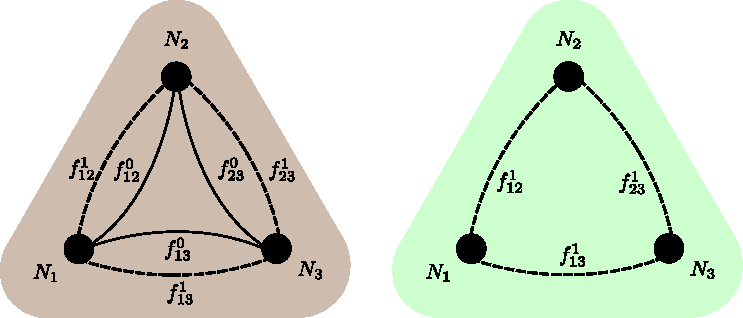
\includegraphics[width=0.8\textwidth]{Figures/3NodeBrownGreen.pdf}
  \end{center}
  \caption{Three node example. \textbf{Left:} Network considering current transmission lines -- solid lines -- and candidate lines -- dashed lines --, brownfield model. \textbf{Right:} Network considering just candidate lines, greenfield model.}
  \label{fig: ThreeNode}
\end{figure}
Luckily, the \textit{dimod} python package from D-Wave allows us to work with two indices so that we do not need to use the previous function to reformulate the problem. 
\subsection{Network Topology}
The TEP problems usually consider the building of new lines in existing connections so that we do not change the network topology. One of the reasons for adding lines in existing connections is because the legal permissions are granted. However, in a future scenario with a high share of decentralized renewable energies, new connections have to be considered. Hence, we are going to enable new connections by changing the topology. Moreover, we allow all lines to be connected to each node, i.e., we are considering fully connected networks.
\subsection{Formulation}
We formulate the TEP problem according to the work of Dilwali \textit{et al.}\,\cite{Dilwali2016} as follows
\begin{mini!}[2]
	{\mathbf{x},\mathbf{g},\mathbf{r},\mathbf{f}^{0},\mathbf{f}^{1}}{\underbrace{\sum_{kl\in C}c_{kl}x_{kl}}_{\textrm{Investment cost}} + \underbrace{\sum_{h\in H}\sum_{k}c_{k}^{(\textrm{oc})}g_{k}(h)}_{\textrm{Operational cost}} + \underbrace{\sum_{h\in H}\sum_{k}r_{k}(h)c_{k}}_{\textrm{Load shedding cost}}}{}{}{\label{eq: objective}}
	\addConstraint{d_{k}(h)-\left(\sum_{l\in E_{k}}f_{kl}^{0}(h) + \sum_{l\in C_{k}}f_{kl}^{1}(h) + g_{k}(h) + r_{k}(h)\right)}{=0\ ,\quad}{\forall k\in N ,h\in H}{\label{const: PowerBalance}}
    \addConstraint{\abs{f_{kl}^{0}(h)} - \bar{f_{kl}^{0}}(h)}{\leq 0\ ,}{\forall\, kl \in E,h\in H }{\label{const: ExistingLimits}}
     \addConstraint{\abs{f_{kl}^{1}(h)} - \bar{f_{kl}^{1}}(h)x_{kl}}{\leq 0\ ,}{\forall\, kl \in C,h\in H }{\label{const: CandidateLimits}}
     \addConstraint{g_{k}(h)-\bar{g}_{k}(h)}{\leq 0\ ,}{\forall\, k\in N,h\in H }{\label{const: BusLimits}}
    \addConstraint{r_{k}(h) - d_{k}(h)}{\leq 0\ ,}{\forall\, k \in N,h\in H }{\label{const: BusLoads}}
    \addConstraint{\mathbf{d}, \mathbf{g}, \mathbf{f}^{0}, \mathbf{f}^{1}}{\geq 0}{}{}
    \addConstraint{x_{kl}}{\in \{0,1\}\ ,}{\forall\, kl \in C,}
\end{mini!}
where the variables are described in Table\,\ref{table:TEPNomenclature}. We next briefly describe each equation:
\begin{itemize}
    \item \textbf{Objective function Eq.\,\eqref{eq: objective}}: it is the sum of investment cost of transmission lines, operational cost of generators and load shedding cost.
    \item \textbf{Power balance Eq.\,\eqref{const: PowerBalance}}: it represents the power balance constraints, i.e., if the demand $d_{k}(h)$ at node $k$ and snapshot $h$ is fulfilled by the generator $g_{k}$ at node $k$ and the power flow incoming from other nodes $f_{kl}^{0}(h)$ and $f_{kl}^{1}(h)$. The term $r_{k}$ is the load shedding. It can be thought of as an artificial generator whose operational cost is very large. It represents the fine for not fulfilling the demand in a node and it guarantees that the problem is feasible. To ensure that mathematically the demand is always fulfilled one can consider a load shedding term that is zero when demand at node $k$ is satisfied by the elements of the network and $r_{k} \neq 0$ when it is not fulfilled. If $r_{k} \neq 0$ the demand is not fulfilled, i.e., the electricity markets cannot offer the required energy to a given node and then pay a fine, which is an extra cost in the objective function. If the load shedding cost is high enough the demand is going to be always fulfilled since the load shedding term is the dominant term we want to minimize.
    \item \textbf{Existing circuit flow limits Eq.\,\eqref{const: ExistingLimits}}: the power flow of an existing transmission $f_{kl}^{0}$ line cannot exceed its maximum capacity, $\bar{f}_{kl}^{0}$.
    \item \textbf{Candidate circuit flow limits Eq.\,\eqref{const: CandidateLimits}}: the power flow of a candidate transmission line $f_{kl}^{1}$ cannot exceed its maximum capacity, $\bar{f}_{kl}^{1}$.
    \item \textbf{Node generation limits Eq.\,\eqref{const: BusLimits}}: the energy produced in a node $k$, $g_{k}$, cannot exceed its maximum energy production, $\bar{g}_{k}$.
    \item \textbf{Node loads limits Eq.\,\eqref{const: BusLoads}}: the load shedding at node $k$, $r_{k}$, cannot exceed the load $d_{k}$ of that node. 
\end{itemize}
\subsection{Remarks}
The previous model is called a transport model since we are not considering Kirchoff's equations. Notice that we include the operational cost which is usually not included in the literature\,\cite{Gomes2019}. The reason for usually not including the operational cost is that other authors consider a single snapshot so that the dominant term is the investment cost. However, if one wants to consider a large number of snapshots, then the operational cost is the dominant term. On the other hand, if we minimize the investment cost, then there is a change of building transmission lines that connect the most expensive generators to the nodes. In summary, extremal solutions lead to a high value of the cost function in one of the following ways:
\begin{itemize}
    \item \textbf{Underinvestment} leads to a high value of the total cost function because the system is not able to fulfill the demand $d(h)$.
    \item \textbf{Overinvestment} leads to a high value of the total cost function even though it satisfies the demand. Intuitively, we are creating more lines $\{x_{kl}\}$ than we need. Usually, there is an upper bound due to the capital budget.
\end{itemize}
The investment cost $c_{kl}$ is the cost of building the transmission line $x_{kl}$ and it is a constant -- we are not considering time-dependent costs. Analogously, the operational cost $c_{j}^{(\textrm{oc})}$ represents the annualised cost per MWh of the produced energy $g_{k}(h)$ at snapshot $h$. For simplicity, we set the operational cost to each carrier -- wind turbine, solar or run of river among others -- to a fixed value -- mean cost of that carrier -- so that we do not have to consider the variation of the cost as function of the node or the time.\\\\
Notice that when the solution is feasible, i.e., $r_k = 0$ for all $k\in N$, then the total cost depends on the investment cost and the operational cost. As stated before, the number of possible configurations of our problem scales badly. For this reason, knowing if we are considering a large set of snapshots -- large investment planning - or a small subset of snapshots gives us clues about what region of the configuration space we should explore. There are two regions to be considered:
\begin{itemize}
    \item \textbf{Large expansion planning:} for instance if we consider a 10 year expansion planning problem and we produce the energy with the cheapest carriers -- e.g. wind turbines -- we will reduce the operational cost drastically as compared with producing the energy with other carriers. However, it is possible that the fact of producing the energy with the cheapest carriers implies the need of building the most expensive transmission lines, hence increasing the investment cost.
    \item \textbf{Short expansion planning:} for instance if we consider a single-snapshot.  Then, it is clear that the minimum total cost function implies a minimum in the investment cost regardless of the operational costs, since the operational costs are lower as compared with the investment cost when there is only one snapshot to optimize over.
\end{itemize}
To summarise, given the energy demand for a set of nodes $N$ for a set of snapshots $H$, the goal is to optimise the network so as to build the minimum amount of transmission lines -- minimizing in that way the investment cost -- while satisfying the energy demand for each snapshot. We are also taking into account the operational cost of each carrier so there is a trade-off between the investment cost of transmission lines and the operational cost of generators used to produce the energy to satisfy the demand.
%%%%%%%%%%%%%%%%%%%%%%%%%%%%%%%%%%%%%%%%%%%%%%%%%%%%%%%%%%%%%%%%%%%%%%%%%%%%%%%%%%
%       SOLVING A SMALL PROBLEM WITH A REAL QUANTUM ANNEALER
%%%%%%%%%%%%%%%%%%%%%%%%%%%%%%%%%%%%%%%%%%%%%%%%%%%%%%%%%%%%%%%%%%%%%%%%%%%%%%%%%%
\section{Small Network solved by D-Wave's simulators}
 We are considering a single snapshot of a three-node fully-connected network with nonexistent lines with a single demand at node $2$ and without the load shedding term. Each node has a single generator $g_{k}$ with a nominal power -- maximum capacity -- of $10$ energy units.
 \begin{table}[H]
\centering
\begin{tabular}{ |c |c| c| }
  \hline			
  \textbf{Symbol} & \textbf{Description} & \textbf{Value}  \\
    \hline		
   $\mathbf{c} = \left[c_{12},c_{13},c_{23}\right]$ & Investment cost & $\left[10, 20, 30\right]$\\
       \hline		
   $\mathbf{c}^{\textrm{oc}} = \left[c_{1}^{\textrm{oc}},c_{2}^{\textrm{oc}}, c_{3}^{\textrm{oc}}\right]$ & Operational cost & $\left[10, 5, 2\right]$\\
          \hline		
   $\mathbf{d} = \left[d_{1}, d_{2}, d_{3}\right]$ & Demands & $\left[0, 12, 0\right]$\\
       \hline		
   $\mathbf{\bar{g}} = \left[\bar{g}_{1},\bar{g}_{2},\bar{g}_{3}\right]$ & Maximum capacity & $\left[10, 10, 10\right]$\\
    \hline	
    $\mathbf{\bar{f}}^{1} = \left[f_{12}^{1},f_{13}^{1},f_{23}^{1}\right]$ & Maximum Power Flow in candidate line & $\left[10, 10, 10\right]$\\
    \hline
\end{tabular}
\caption{Investment cost, operational cost, demand, maximum capacity per generator and maximum power flow per candidate line for a three node network.}
\label{tab:SmallNetwork}
\end{table}
We use synthetic data for our TEP problem described in Table\,\ref{tab:SmallNetwork}.\\
The objective function for the three node fully connected network described above is
\begin{mini!}[2]
	{\mathbf{x}, \mathbf{g}}{\underbrace{\mathbf{C}^{\intercal}\mathbf{x}}_{\textrm{Investment Cost}} + \underbrace{\mathbf{C}_{\textrm{oc}}^{\intercal}\mathbf{g}}_{\textrm{Operational Cost}}}{}{}{}
 	\addConstraint{g_{k}}{\leq \bar{g}_{k} }{\forall\, k \in N}{}
	\addConstraint{d_{k}}{= g_{k}  + \underbrace{\sum_{l\neq k, l\in N}g_{k}x_{kl}}_{\textrm{Quadratic Constraint}}}{\forall\, k \in N}{}
    \addConstraint{\mathbf{d}, \mathbf{g}}{\geq 0\,}{}{}
    \addConstraint{x_{kl}}{\in \{0,1\},\,}{\forall\, kl \in C}.
    \end{mini!}
Notice that we are not considering the power flow limits $f_{kl}^{1}$ of candidate lines. Any candidate line can transmit any amount of energy. In other words, we wrote the problem in such a way that none of the power flow limits is going to be violated, see Figure\,\ref{fig: Green_inital}.
\begin{figure}[H]
  \begin{center}
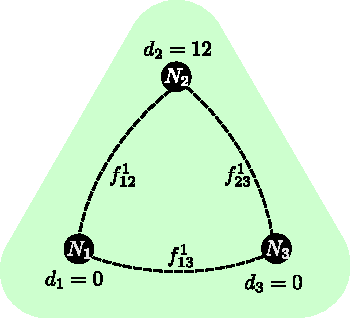
\includegraphics[width=0.4\textwidth]{Figures/Green_Initial.pdf}
  \end{center}
  \caption{Graphic formulation of three node problem.}
  \label{fig: Green_inital}
\end{figure}
The demand at node $2$ is $12$ energy units, so it cannot be fulfilled by its own generator and requires energy from at least one of the neighboring nodes which means we need to build at least one transmission line connected to node $2$. The results are going to be presented in next chapter.
%%%%%%%%%%%%%%%%%%%%%%%%%%%%%%%%%%%%%%%%%%%%%%%%%%%%%%%%%%%%%%%%%%%%%%%%%%%%%%%%%%
%       BENDERS DECOMPOSITION for TEP [Large Problems]
%%%%%%%%%%%%%%%%%%%%%%%%%%%%%%%%%%%%%%%%%%%%%%%%%%%%%%%%%%%%%%%%%%%%%%%%%%%%%%%%%%
\section{Benders Decomposition in TEP}
In Chapter\,\ref{Chapter3} we showed three hybrid approaches that combine classical and quantum solvers. In this work, we decided to explore the Benders' decomposition approach due to two main points. Firstly, the convergence properties of Benders' decomposition allows us to know how good a solution is. Secondly, TEP problems have diagonal structure which means they are suitable for a Benders' decomposition approach. We propose a quantum Benders' decomposition scheme for a general formulation of TEP problems, but its implementation is left for a future work. However, we present the results of a few TEP problem solved by D-Wave hybrid solvers. These results will be be compared in the future with the results we get from our quantum BD algorithm.\\\\\
In order to simplify the problem we consider a single snapshot so that we can drop the $h$ index. As discussed in Ch.\,\ref{Chapter3}, we can formulate the problem by maximizing a dual function or by minimizing the primal problem with the dual as penalties. The Benders' decomposition algorithm that we propose consists of four steps:
\begin{itemize}
    \item \textbf{Step 1} (\textit{Initialization of Benders’ decomposition})\textbf{:} we initialize the iteration counter $t$, the upper bound $\bar{z}^{0}$, the lower bound $\underline{z}^{0}$, the load shedding and operational cost $\alpha^{0}$ and the penalty term associated with the violation of power flow constraints of candidate lines $\Pi_{f_{kl}^{1}}$.
    \item \textbf{Step 2} (\textit{Master problem solved by a quantum annealer})\textbf{:} we increase the lower bound $\underline{z}^{t}$ by taking the minimum value of 
        \begin{mini!}[2]
	   {\mathbf{x}}{\underline{z}^{t}}{}{}{}
	   \addConstraint{\underline{z}^{t} \geq \sum_{kl\in C}c_{kl}x_{kl}^{t} + \alpha^{t-1} - \underbrace{\sum_{kl\in C}\Pi^{\tau}_{f_{kl}^{1}}\left(x_{kl}^{t} - x_{kl}^{\tau}\right)}_{\textrm{Benders' cuts}}}{=0,}{\quad \forall \tau = 1,\hdots,t-1.}{}
        \end{mini!}
    In that equation $\alpha^{t-1}$ represent the summation of the objective function of the slave problem(s) and $\Pi_{f_{kl}^{1}}^{\tau}$ represent the Benders' cut of iteration $\tau$ where $\tau < t$, for the linking constraint of Eq.\,\eqref{const: CandidateLimits}. Notice that we have a Benders' cut for every candidate circuit flow constraint $f_{kl}^{1}$. In every iteration of Benders' algorithm we are adding cuts, in other words we are restricting the region of feasible solutions.
    \item \textbf{Step 3} (\textit{Slave problem solved by a classical solver})\textbf{:} we minimize $\alpha^{t}$ which includes the load shedding cost and the operational cost.
    \begin{mini!}[2]
	{\mathbf{g},\mathbf{r}, \mathbf{f}^{0}, \mathbf{f}^{1}}{\alpha^{t} \equiv \underbrace{\sum_{k}c_{k}^{(\textrm{oc})}g_{k}}_{\textrm{Operational cost}} + \underbrace{\sum_{k}r_{k}c_{k}}_{\textrm{Load shedding cost}}}{}{}{}
	\addConstraint{d_{k}-\left(\sum_{l\in E_{k}}f_{kl}^{0} + \sum_{l\in C_{k}}f_{kl}^{1} + g_{k} + r_{k}\right)}{=0,\quad}{\forall k\in N }{}
    \addConstraint{\abs{f_{kl}^{0}} - \bar{f}_{kl}^{0}}{\leq 0,\,}{\forall\, kl \in E}{}
     \addConstraint{\abs{f_{kl}^{1}} - \bar{f}_{kl}^{1}x^{t}_{kl}}{\leq 0,\,}{\forall\, kl \in C}{}
     \addConstraint{g_{k}-\bar{g}_{k}}{\leq 0,\,}{\forall\, k\in N}{}
    \addConstraint{r_{k} - d_{k}}{\leq 0,\,}{\forall\, k \in N}{}
    \addConstraint{\mathbf{d}, \mathbf{g}, \mathbf{f}^{0}, \mathbf{f}^{1}}{\geq 0\,}{}{\label{const: positivevalues}}.
    \end{mini!}
    \item \textbf{Step 4} (\textit{Stopping criterion})\textbf{:} after minimizing $\alpha^{t}$ we reduce the upper bound
    \begin{equation}
        \bar{z}^{t} = \min \{\bar{z}^{t-1}, \sum_{kl \in C}c_{kl}x_{kl}^{t} + \alpha^{t}\}.
    \end{equation}
    If the difference between the upper and lower bound is less or equal than a given threshold
    \begin{equation}
        \bar{z} - \underline{z} \leq \epsilon,
    \end{equation}
    then the Benders' algorithm stops and outputs the value of $\{\mathbf{x},\mathbf{g},\mathbf{r},\mathbf{f^{1}}\}$ as the (sub-)optimal solution. Otherwise, it goes to step 2 with the new candidate solution as input.
\end{itemize}

